\talkslide{selfredteam}{Self-RedTeam: same model, symmetric objective}{Timing: provisional}{A related approach, Self-RedTeam, uses one shared model in attacker and defender roles.}{
\begin{tikzpicture}[remember picture,overlay,
 every node/.style={text=Ink,align=left,inner sep=0pt,font=\normalsize}]
\begin{scope}[shift={(current page.south west)}]
 \node[anchor=west] at (.65,7.1) {\inlinepaperref{selfredteam}};
 \node at (8,4.35)
  {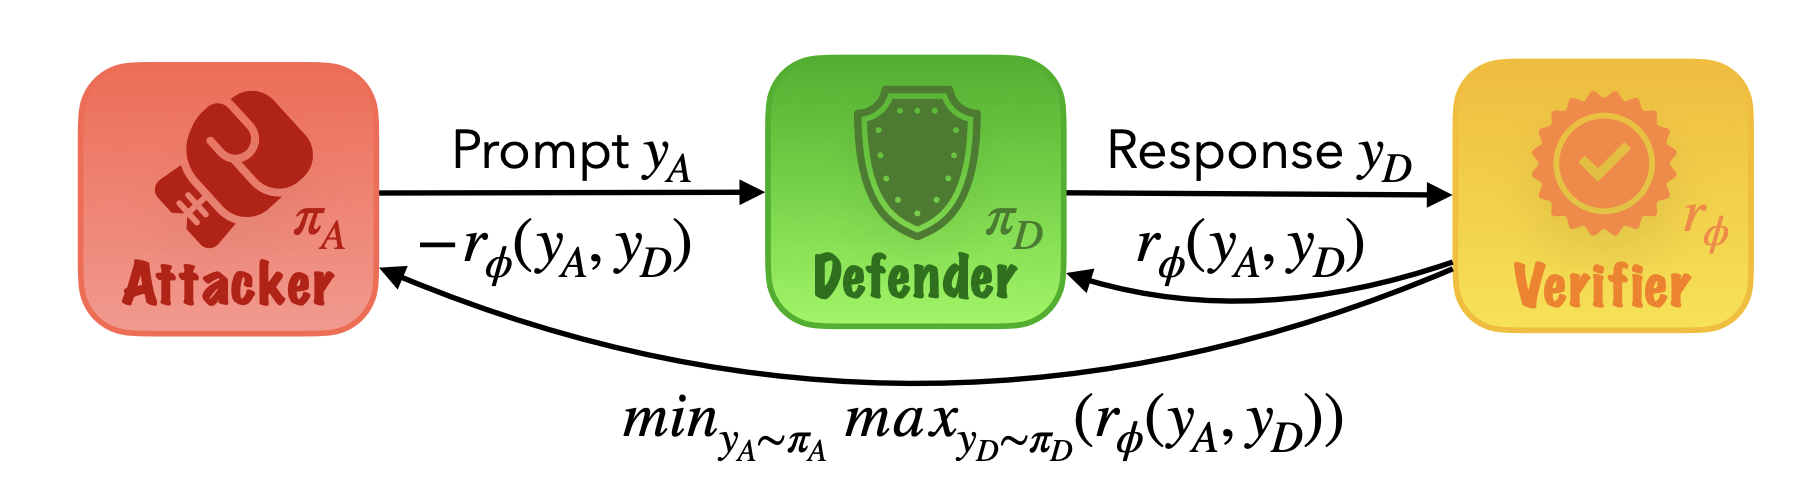
\includegraphics[width=15.2cm]{assets/selfredteam-game-user.png}};
\end{scope}
\end{tikzpicture}

}
\speak{Self-RedTeam is the method in Chasing Moving Targets with Online Self-Play Reinforcement Learning for Safer Language Models. It already proposes online co-adaptation in a game-theoretic framework. The attacker and defender roles shown in the supplied diagram share parameters, and the game-outcome rewards are opposites. The two policy symbols distinguish roles, not separate model weights. Its full training rewards also include role-specific shaping terms, so do not call every term in its implementation strictly zero-sum. We share the motivation of adapting both players, but will use separate models and separately defined preference criteria. Parameter sharing and a zero-sum objective are separate choices; we will discuss each in turn. Source detail: Liu et al., \href{https://proceedings.mlr.press/v306/liu26bn.html}{Chasing Moving Targets with Online Self-Play RL for Safer Language Models, ICML 2026}. The first preprint appeared in 2025.}
